\documentclass{article}
\usepackage[T1]{fontenc}
\usepackage{frutiger}
\usepackage{microtype}
\DisableLigatures[f]{encoding=T1}% Disable ligatures because font doesn't have it
\usepackage{amsmath,amsfonts,amssymb,amsthm} % Math packages

\usepackage{xcolor}
\usepackage{graphicx}
\usepackage{circuitikz}[european]

%% the following commands are needed for some matlab2tikz features
\usepackage{tikz}
\usepackage{pgfplots}
\usepackage{siunitx}
\pgfplotsset{compat=newest}
\usepgfplotslibrary{fillbetween}
\usetikzlibrary{plotmarks}
\usetikzlibrary{arrows.meta}
\usepgfplotslibrary{patchplots}
\usepackage{grffile}
% Tikz
\usetikzlibrary{shapes}
\usetikzlibrary{calc, intersections, arrows, shapes}

\usetikzlibrary{external}
\usetikzlibrary{decorations.markings}
\tikzexternalize[prefix=pdf/]

\definecolor{fhggreen}{RGB}{23,200,90}
\definecolor{fhggrey}{RGB}{225,227,227}

\renewcommand{\familydefault}{\sfdefault}
\usepackage[cm]{sfmath}


\begin{document}
\tikzsetnextfilename{gridmodel_sim}
\definecolor{fhggrey}{RGB}{225,227,227}

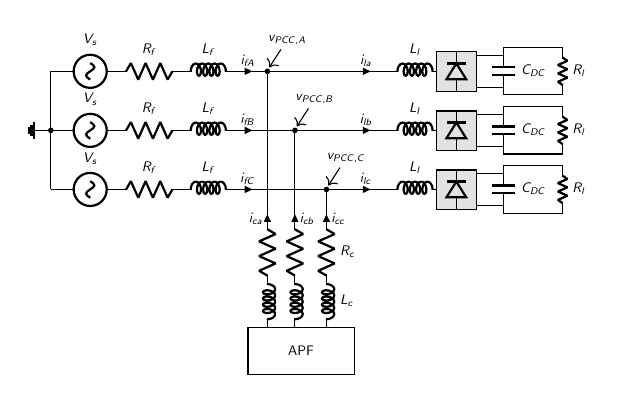
\begin{tikzpicture}[scale = 0.5, transform shape]
    %\draw (-1,1) node[draw,circle,fill=white,minimum size=30pt]{$V_f$};
    \draw (-1.5,0) to[short] (-1,0) to[sV, l^=$V_{s}$] (0,0) to[R=$R_f$] (2,0) to [L=$L_f$] (3,0) 
    	to[short, i^>=$i_{fC}$] (4,0) to (5.5,0) to[short, *-] (5.5,-.5) to[short, i^<=$i_{cc}$] (5.5,-1) 
    	to[R=$R_c$] (5.5,-2.2) to[L= $L_c$] (5.5,-3.5);
    \draw (-1.5,1.5) to[short,*-](-1,1.5) to[sV, l^=$V_{s}$] (0,1.5) to[R=$R_f$] (2,1.5) to [L=$L_f$] (3,1.5) 
    	to[short, i^>=$i_{fB}$] (4,1.5) to (4.7,1.5) to[short, *-] (4.7,-.5) to[short, i^<=$i_{cb}$] (4.7,-1)
    	to[R] (4.7,-2.2) to[L] (4.7,-3.5);
    \draw (-1.5,3) to[short] (-1,3) to[sV, l^=$V_{s}$] (0,3) to[R=$R_f$] (2,3) to [L=$L_f$] (3,3) 
    	to[short, i^>=$i_{fA}$] (4,3) to[short, *-] (4,-.5) to[short, i_<=$i_{ca}$] (4,-1) 
    	to[R] (4,-2.2) to[L] (4,-3.5);
    \draw (3.5,-3.5) 
    	node[draw,minimum width=2.7cm,minimum height=1.2cm,anchor=north west]{ APF};
\draw (-1.5,0) to[short] (-1.5,3);
	\draw (-1.5,1.5) node[ground, rotate=270]{};% to[short] (-1.5,1.5);   	
   	\draw (4.7,0) to (6,0)  to[short, i^>=$i_{lc}$] (7,0) to[L=$L_{l}$]  (8.5,0);
   	\draw (4.5,1.5) to[short] (6,1.5) to[short, i^>=$i_{lb}$] (7,1.5) to[L=$L_{l}$] (8.5,1.5);
   	\draw (4,3) to[short] (6,3) to[short, i^>=$i_{la}$] (7,3) to[L=$L_{l}$] (8.5,3);
   	\draw (8.3,3.5) node[draw,fill=fhggrey,minimum width=1cm,minimum height=1cm,anchor=north west]{};
   	\draw (8.8, 2.5) to[/tikz/circuitikz/bipoles/length=1cm,Do] (8.8,3.5);
   	\draw (8.3,2) node[draw,fill=fhggrey,minimum width=1cm,minimum height=1cm,anchor=north west]{};
   	\draw (8.8, 1) to[/tikz/circuitikz/bipoles/length=1cm,Do] (8.8,2);
   	\draw (8.3,0.5) node[draw,fill=fhggrey,minimum width=1cm,minimum height=1cm,anchor=north west]{};
   	\draw (8.8, -0.5) to[/tikz/circuitikz/bipoles/length=1cm,Do] (8.8,0.5);
   	%\draw (8.5,3.5)
   		%node[draw,minimum width=1.5cm,minimum height=4cm,anchor=north west,fill=white]{};
   	\draw (9.3,3.4) to[short] (10,3.4) to[/tikz/circuitikz/bipoles/length=1cm,C,l^=$C_{DC}$] (10,2.6) to[short] (9.3,2.6);
   	\draw (10,3.4) to[short] (10,3.6) to[short] (11.5,3.6) to[/tikz/circuitikz/bipoles/length=0.8cm,R=$R_l$] (11.5,2.4) to[short] (10,2.4) to[short] (10,2.6);
   	\draw (9.3,1.9) to[short] (10,1.9) to[/tikz/circuitikz/bipoles/length=1cm,C,l^=$C_{DC}$] (10,1.1) to[short] (9.3,1.1);
   	\draw (10,1.9) to[short] (10,2.1) to[short] (11.5,2.1) to[/tikz/circuitikz/bipoles/length=0.8cm,R=$R_l$] (11.5,.9) to[short] (10,.9) to[short] (10,1.1);
   	\draw (9.3,0.4) to[short] (10,0.4) to[/tikz/circuitikz/bipoles/length=1cm,C,l^=$C_{DC}$] (10,-0.4) to[short] (9.3,-0.4);
   	\draw (10,0.4) to[short] (10,0.6) to[short] (11.5,.6) to[/tikz/circuitikz/bipoles/length=0.8cm,R=$R_l$] (11.5,-.6) to[short] (10,-.6) to[short] (10,-.4);
   	
   	\node (vfa) at (4.5,3.8) {$v_{PCC,A}$};
   	\node (vfb) at (5.2,2.3) {$v_{PCC,B}$};
   	\node (vfc) at (6,0.8) {$v_{PCC,C}$};
   	\draw[->] (vfa) -- (4.05,3.1);
   	\draw[->] (vfb) -- (4.75,1.6);
   	\draw[->] (vfc) -- (5.55,0.1);

   	
\end{tikzpicture}
\end{document}